
\documentclass[12pt,epsfig,color,russian]{article}
\usepackage[russian]{babel}
\usepackage{epsfig}
\usepackage{color}

\topmargin=0cm
\hoffset -30mm
\voffset -20mm
\setlength{\unitlength}{1mm}
\parindent=10mm
\textheight=260mm
\textwidth=185mm
\pagestyle{empty}

\begin{document}
\sf\Large
\centerline{\LARGE\bf Распределение Максвелла}

Сначала поговорим о вероятности и введем несколько новых понятий из математической статистики. Для наглядности рассмотрим пример.

\noindent
\begin{picture}(190,40)(0,0)
 %\put(0,0){\framebox(190,40)[b]{}}
 \put(0,0){\includegraphics{GP009F1a.eps}}
 \put(70,35){\makebox(0,0)[tl]{\parbox{115mm}{
    Пусть есть некий объем $V_r$, и в нем случайно мечется муха. Сфотографируем какую-то часть этого объема $dV_r=dx\cdot dy\cdot dz$. Тогда вероятность обнаружить муху на снимке пропорциональна $dV_r$. То есть, в вероятность
}}}
\end{picture}\\
должен входить {\bf Space Factor} -- отношение объемов
    \begin{equation}\label{Eq.Volumes}
   \mathcal{F}=\frac{\texttt{интересующий нас объем}}{\texttt{весь возможный объем}}=
   \frac{dV_r}{V_r}
   \end{equation}

Кроме координат $\vec{r}$=($x$,$y$,$z$), у мухи есть еще и скорость: $\vec{v}$=($v_x$,$v_y$,$v_z$). При этом, аналогично тому, как координаты ограничены объемом $V_r$, так же и составляющие скорости ограничены каким-то ``объемом'' $V_v$ в ``про\-с\-транстве скоростей'':\vspace{-5mm}
\begin{displaymath}
\begin{array}{ccc}
 -v_0\leq& v_x &\leq +v_0\\
 -v_0\leq& v_y &\leq +v_0\\
 -v_0\leq& v_z &\leq +v_0
\end{array}
\end{displaymath}
где $v_0$ -- максимальная скорость, на которую муха способна.

Предположим теперь, что наш фотоаппарат -- особенный и обладает избирательностью к скоростям. Тогда портрет мухи удачен только тогда, когда, во-первых, ее координаты попали в объемчик $dV_r$, и, во-вторых, скорость ее -- не любая, а тоже лежит в пределах ``скоростного объемчика'' $dV_v=dv_x\cdot dv_y\cdot dv_z$:\\
\begin{picture}(190,70)(0,0)
 %\put(0,0){\framebox(190,70)[b]{}}
 \put(10,0){\includegraphics{GP009F1b.eps}}
\end{picture}\\
Понятие {\bf Фазовый объем} -- в зависимости от задачи, это может быть только $dV_r$, или только $dV_v$, но чаще это их произведение $dV=dV_r\cdot dV_v = dx\cdot dy\cdot dz\cdot dv_x\cdot dv_y\cdot dv_z$. Тогда вероятность вместо отношения {\bf объемов} в формуле (\ref{Eq.Volumes}) будет включать в себя отношение {\bf фазовых объемов:}
    \begin{equation}\label{Eq.PhaseVolumes}
   \mathcal{F}=\frac{\texttt{интересующий нас фазовый объем}}{\texttt{весь возможный фазовый объем}}=
   \frac{dV_r\cdot dV_v}{V_r\cdot V_v}
   \end{equation}
(по-английски это называется {\bf Phase Space Factor}).\\

\noindent
Теперь усложним условия для мухи. Представим, что объем ее оби\-та\-ния $V_r$ не совсем однороден, а какие-то его части для мухи более при\-тя\-га\-тель\-ны -- например, где-то намазано медом, причем, чем правее -- тем больше. $\Rightarrow$ мы должны ввести еще одно понятие -- {\bf плотность вероятности $\bf f$}\\ (фун\-к\-цию, в соответствии с которой намазан мед). Она характеризует как бы относительный ``вес'' разных точек пространства, как обычного, так и скоростного. Это значит, что вообще-то $f=f(\vec{r},\vec{v})$.\\
\begin{picture}(190,38)(0,0)
 %\put(0,0){\framebox(190,38)[b]{}}
 \put(0,0){\includegraphics{GP009F1c.eps}}
 \put(70,35){\makebox(0,0)[tl]{\parbox{115mm}{
 В нашем примере справа меду больше, чем слева, то есть, $f=kx$. Как результат, муху неудержимо будет тянуть вправо. Так же и какие-то скорости могут оказаться для мухи более предпочтительными.
}}}
\end{picture}\\
Итак, вероятность качественно сфотографировать муху пропорциональна не только фазовому объему фотографии, но и плотности вероятности:
\begin{displaymath}
 d\mathcal{W}\sim f(\vec{r},\vec{v})\cdot dV_r\cdot dV_v
\end{displaymath}
Если ``фотографируется'' относительно большой фазовый объем $V_\phi$, в пределах которого $f$ существенно меняется, то надо проинтегрировать $f$ по этому объему:
\begin{displaymath}
 \mathcal{W}\sim \int\limits_{V_\phi}f(\vec{r},\vec{v})\cdot dV_r\cdot dV_v
\end{displaymath}

И последний штрих: нормировка, т.е, равенство единице интеграла по {\bf всему} (а не фотографируемому) фазовому объему. Отсюда следует:
\begin{displaymath}
 \mathcal{W}=\left[\int\limits_{V_\phi}f(\vec{r},\vec{v})\cdot dV_r\cdot dV_v\right]/
\left[\int\limits_{V}f(\vec{r},\vec{v})\cdot dV_r\cdot dV_v\right]
\end{displaymath}


%\newpage
Мы знаем, что пространство -- однородно. Поэтому движение по каждой из осей ($x,y,z$) происходит независимо. Рассмотрим только одну из этих осей, например, ось $x$. Для каждой молекулы величина $v_x$ может быть от $-\infty$ до $+\infty$. Поскольку пространство -- не только однородно, но еще и изотропно, то направления $+$ и $-$ также полностью равноправны. Таким образом, распределение вероятности должно быть четной функцией.\\
\begin{picture}(190,65)(0,0)
 %\put(0,0){\framebox(190,60)[b]{}}
 \put(0,0){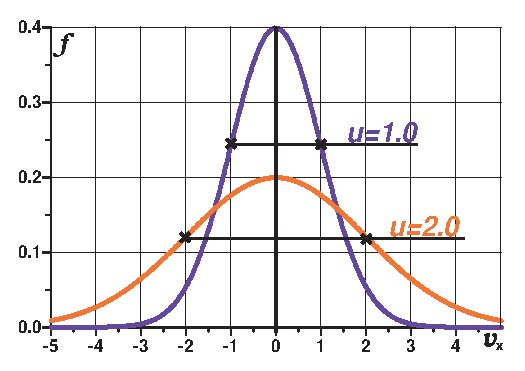
\includegraphics{GP009F02.eps}}
 \put(87,62){\makebox(0,0)[tl]{\parbox{100mm}{
Логично предположить, что, как это характерно для всяких СЛУЧАЙНЫХ процессов, это распределение яв\-ля\-ет\-ся НОРМАЛЬНЫМ, т.е., описывается функцией Гаусса:\vspace{-7mm}
\begin{equation}\label{Eq.Gauss}
f(v_x)=A\cdot \exp\left(-\frac{v_x^2}{2u^2}\right)\vspace{-2mm}
\end{equation}
где величина $u$ -- дисперсия этого распределения, а амплитуда $A$ должна }}}
\end{picture}\\
 быть такой, чтобы выполнялось условие нормировки (т.е., чтобы суммар\-ная вероятность равнялась 1). Физический смысл $f(v_x)$: если мы хотим найти вероятность того, что $x$-составляющая скорости молекулы лежит в интервале от $v_x$ до $v_x$+$dv_x$, надо просто величину этого интервала (или, иначе, фазового объема) $dv_x$ умножить на плотность вероятности $f(v_x)$:
\begin{equation}
df(v_x)=f(v_x)dv_x=A\cdot \exp\left(-\frac{v_x^2}{2u^2}\right)\cdot dv_x
\end{equation}
Если нас интересует не малый фазовый объемчик $dv_x$, а большой интервал от $v_1$ до $v_2$, то надо проинтегрировать $df(v_x)$ по этому интервалу. Анало\-ги\-чно дело обстоит с $v_y$ и $v_z$:
\begin{equation}
df(v_y)=A\cdot \exp\left(-\frac{v_y^2}{2u^2}\right)\cdot dv_y,\;\;\;\;\;\;\;
df(v_z)=A\cdot \exp\left(-\frac{v_z^2}{2u^2}\right)\cdot dv_z.
\end{equation}
Из соображений однородности пространства следует, что и амплитуда $A$, и дисперсия $u$ во всех 3 случаях -- одни и те же. Чему они равны? {\bf Условие нормировки} (включает в себя интеграл Пуассона):
\begin{displaymath}
1=\int\limits_{-\infty}^{+\infty}f(v_x)dv_x=
\int\limits_{-\infty}^{+\infty}A\cdot\exp\left(-\frac{v_x^2}{2u^2}\right)dv_x
\end{displaymath}
\newpage
Интеграл Пуассона:\hfill{ }{\LARGE\sl ПРИЛОЖЕНИЕ}
\begin{displaymath}
I=\int\limits_{-\infty}^{+\infty}\exp\left(-\frac{x^2}{2\sigma^2}\right)dx=?
\end{displaymath}
``индейская хитрость'': вместо $I$ вычислим $I^2$, а потом возьмем из него корень.
\begin{displaymath}
I^2=\int\limits_{-\infty}^{+\infty}\exp\left(-\frac{x^2}{2\sigma^2}\right)dx\cdot
    \int\limits_{-\infty}^{+\infty}\exp\left(-\frac{y^2}{2\sigma^2}\right)dy
\end{displaymath}
Если теперь считать, что $x$ и $y$ -- не просто переменные, а декартовы координаты, то
вместо произведения двух интегралов получается один интеграл по плоскости:
\begin{displaymath}
I^2=\int\limits_{-\infty}^{+\infty}\int\limits_{-\infty}^{+\infty}\exp\left(-\frac{x^2+y^2}{2\sigma^2}\right)dx\;dy
\end{displaymath}
Заметим, что $dx\cdot dy$ есть ни что иное как элемент площади $dS$, а $x^2+y^2$ -- это длина радиуса $r^2$:
\begin{displaymath}
I^2=\int\limits_S\exp\left(-\frac{r^2}{2\sigma^2}\right)dS
\end{displaymath}
Теперь вторая ``индейская хитрость''. Перейдем от декартовых к полярным координатам $r$ и $\varphi$, причем элемент площади в этом случае $dS=r\cdot dr\cdot d\varphi$, а интегрировать теперь надо по $\varphi$ от 0 до $2\pi$, а по $r$ от 0 до $\infty$:
\begin{displaymath}
I^2=\int\limits_0^{2\pi}d\varphi\int\limits_0^\infty\exp\left(-\frac{r^2}{2\sigma^2}\right)r\cdot dr
\end{displaymath}
Интеграл по $\varphi$ равен $2\pi$, а интеграл по $r$ легко берется при замене переменной $(-r^2/2\sigma^2)\rightarrow (z)$. При этом, $r\cdot dr=-dz\cdot\sigma^2$:
\begin{displaymath}
I^2=-2\pi\sigma^2\int\limits_0^{-\infty}\exp\left(z\right) dz = -2\pi\sigma^2\cdot e^z|_0^{-\infty}=2\pi\sigma^2
\end{displaymath}
Таким образом, искомое значение интеграла: \fbox{$I=\sigma\sqrt{2\pi}$}.
\newpage
Итак, вернемся к распределению молекул по скоростям. Из условия нормировки следует:\vspace{-5mm}
\begin{equation}
1=A\cdot u\sqrt{2\pi}\hspace{10mm}\Rightarrow\hspace{10mm}A=\frac{1}{u\sqrt{2\pi}}
\end{equation}
Из свойств нормального распределения  известно, что входящая в формулу (\ref{Eq.Gauss}) дисперсия $u$ представляет собой среднеквадратичное отклонение аргу\-мен\-та от центра распределения.  Но об этом -- позже. Пока считаем, что это -- просто какой-то параметр.

Вспомним, что все сказанное справедливо не только для $v_x$, но и для $v_y$, $v_z$. Поскольку, как уже говорилось, пространство однородно, то все эти распределения независимы. Поэтому, вероятность того, что молекула имеет конкретную скорость $\vec{v}$, равна ПРОИЗВЕДЕНИЮ вероятностей по каждой составляющей $df(v_x)$, $df(v_y)$ и $df(v_z)$:
\begin{displaymath}
df(\vec{v})=df(v_x)\cdot df(v_y)\cdot df(v_z)
 =f(v_x)dv_x\cdot f(v_y)dv_y\cdot f(v_z)dv_z
\end{displaymath}
Подставив в качестве $f(v_i)$ нормальные распределения (\ref{Eq.Gauss}), получим $df(\vec{v})$ -- вероятность того, что вектор $\vec{v}$ заканчивается в маленьком ``кубике'' фазового объема $dV_v=dv_x\cdot dv_y\cdot dv_z$:\vspace{-2mm}
\begin{equation}\label{Eq.Maxwell_1_vec{v}}
df(\vec{v})
 =\frac{1}{\left(u\sqrt{2\pi}\right)^3}\cdot \exp\left(-\frac{v^2}{2u^2}\right)\cdot dV_v
\end{equation}
Если нас интересует не конкретное направление вектора $\vec{v}$, а только его абсолютная величина $v$, то надо это выражение проинтегрировать по всем углам. Для этого опять перейдем от декартовой к полярной системе ко\-ор\-ди\-нат, учитывая, что в ней элемент фазового объема $dV_v$ выражается как $dV_v=v^2\cdot\sin\vartheta\cdot d\vartheta\cdot d\varphi\cdot dv$:
\begin{displaymath}
df(v)=\int\limits_{\varphi=0}^{2\pi}\int\limits_{\vartheta=0}^\pi
 \frac{1}{\left(u\sqrt{2\pi}\right)^3}\cdot \exp\left(-\frac{v^2}{2u^2}\right)v^2\cdot\sin\vartheta\cdot d\vartheta\cdot d\varphi\cdot dv
\end{displaymath}
Проинтегрировав по $\vartheta$ и $\varphi$, получим \underline{\color{blue}\bf распределение Максвелла}\\ (James Clerk Maxwell 1831-1879, Эдинбург):
\begin{equation}\label{Eq.Maxwell_1}
df(v)= \frac{4\pi}{\left(u\sqrt{2\pi}\right)^3}\cdot \exp\left(-\frac{v^2}{2u^2}\right)v^2\cdot dv
\end{equation}
\newpage
Итак, перед нами \underline{\color{blue}\bf распределение Максвелла}\\ (James Clerk Maxwell 1831-1879, Эдинбург):
\begin{equation}\
df(v)= \frac{4\pi}{\left(u\sqrt{2\pi}\right)^3}\cdot \exp\left(-\frac{v^2}{2u^2}\right)v^2\cdot dv
\end{equation}
\begin{picture}(190,63)(0,0)
 %\put(0,0){\framebox(190,60)[b]{}}
 \put(0,0){\includegraphics{GP009F03.eps}}
\end{picture}\\
По оси абсцисс отложена относительная скорость молекул (скорость в единицах $u$), а по оси ординат -- плотность вероятности. Чтобы найти отсюда вероятность того, что у пойманной молекулы скорость окажется, например, в интервале от 1.5$u$ до 2.0$u$, нужно проинтегрировать плотность вероятности по ин\-те\-ре\-су\-ю\-ще\-му нас фазовому объему, то есть, вычислить интеграл
\begin{displaymath}
\mathcal{W}(1.5u\leq v\leq2.0u)=\int\limits_{v=1.5u}^{2.0u}f(v)dv
\end{displaymath}


Для полной ясности осталось показать, что же такое $u$. Для этого вычислим средний квадрат скорости {\color{green}$\overline{v^2}$}:
\begin{equation}\label{Eq.v^2_1}
{\color{green}\overline{v^2}}\equiv\frac{\int\limits_0^\infty {\color{green}v^2}\cdot f(v)\;dv}
                         {\int\limits_0^\infty f(v)\;dv}=
\frac{\int\limits_0^\infty {\color{green}v^2}\cdot\exp\left(-\frac{v^2}{2u^2}\right) \cdot v^2\;dv}
                         {\int\limits_0^\infty \exp\left(-\frac{v^2}{2u^2}\right) \cdot v^2\;dv}
\end{equation}
Интеграл $I$, стоящий в числителе, берем по частям $\left(\int XdY=XY-\int YdX\right)$, полагая $Y$=$-u^2\exp\left(-\frac{v^2}{2u^2}\right)$, $X$=$v^3$. Тогда $dY=\exp\left(-\frac{v^2}{2u^2}\right)v\;dv$, $dX=3v^2dv$, а искомый интеграл $I$ равен
\begin{displaymath}
I=\int\limits_{v=0}^\infty XdY = \left.XY\right|_{v=0}^\infty\;\;-\int\limits_{v=0}^\infty YdX =
\end{displaymath}
\begin{displaymath}
 =\left.-u^2v^3\exp\left(-\frac{v^2}{2u^2}\right)\right|_{v=0}^\infty\;\;
 +3u^2\int\limits_{v=0}^\infty\exp\left(-\frac{v^2}{2u^2}\right)v^2\;dv
\end{displaymath}
Первое из двух слагаемых =0, а второе включает в себя такой же интеграл, что стоит в знаменателе дроби (\ref{Eq.v^2_1}), и он к нашей радости сокращается! Таким образом, получаем, что ${\color{green}\overline{v^2}}={\color{green}3u^2}$. Поскольку $\frac{m\overline{v^2}}2$ есть ни что иное как средняя кинетическая энергия молекулы $\overline{w}$, равная, как мы знаем, $\frac32kT$, то
\begin{equation}
{\color{green}u^2}=\frac{\overline{v^2}}3=\frac{2\overline{w}}{3m}= \frac{2\cdot3\;kT}{3\cdot2\;m}={\color{green}\frac{kT}m}
\end{equation}
Подставив найденное значение $u^2=kT/m$ в уравнение (\ref{Eq.Maxwell_1}), получим {\color{blue}\bf распределение Максвелла} уже без всяких неизвестных параметров:
\begin{equation}{\color{blue}
df(v)= 4\pi\left(\frac{m}{2\pi kT}\right)^{3/2}\cdot \exp\left(-\frac{mv^2}{2kT}\right)v^2\cdot dv
}
\end{equation}

По аналогии со средне-квадратичной, можно вычислить скорость, сре\-д\-нюю по модулю, среднюю
по какой-то составляющей, и т.д. Например, средняя по модулю скорость {\color{red}$\overline{v}$} равна:
\begin{displaymath}
{\color{red}\overline{v}}\equiv\frac{\int\limits_0^\infty {\color{red}v}\cdot f(v)\;dv}
                         {\int\limits_0^\infty f(v)\;dv}=
4\pi\left(\frac{m}{2\pi kT}\right)^{3/2}\cdot
\frac{\int\limits_0^\infty {\color{red}v}\cdot\exp\left(-\frac{v^2}{2u^2}\right) \cdot v^2\;dv}
                         {\int\limits_0^\infty f(v)\;dv}
\end{displaymath}
Интегрируя по частям числитель, получим
\begin{displaymath}
 \texttt{числитель}=\left.-u^2v^2\exp\left(-\frac{v^2}{2u^2}\right)\right|_{v=0}^\infty\;\;
 +2u^2\int\limits_{v=0}^\infty\exp\left(-\frac{v^2}{2u^2}\right)v\;dv=
\end{displaymath}
(замена переменной: $(-v^2/2u^2)\rightarrow t; \;\;\; dt=-v\,dv/u^2$)
\begin{displaymath}
=0\;-2u^4\int\limits_{t=0}^{-\infty}e^tdt=2u^4
\end{displaymath}
Знаменатель же по условиям нормировки просто обязан равняться 1. Поэтому для  {\color{red}$\overline{v}$} получаем:
\begin{displaymath}
{\color{red}\overline{v}}=
4\pi\left(\frac{m}{2\pi kT}\right)^{\frac32}\cdot2u^4=4\pi\left(\frac{m}{2\pi kT}\right)^{\frac32}\cdot\frac{2k^2T^2}{m^2}={\color{red}\sqrt{\frac{8kT}{\pi m}}}
=u\sqrt{\frac{8}{\pi}}\simeq1.60u
\end{displaymath}
Мы уже вычисляли {\color{green}$\overline{v^2}$} и получили, что $\overline{v^2}=3u^2$. Подставив $kT/m$ вместо $u^2$, получим средне-квадратичную скорость:
\begin{displaymath}
{\color{green}\sqrt{\overline{v^2}}}={\color{green}\sqrt{\frac{3kT}{m}}}=u\sqrt{3}\simeq1.73u
\end{displaymath}
Можно еще найти наиболее вероятную скорость {\color{magenta}$v_p$}.  Для этого ищем точку максимума на кривой $f(v)$, приравяв нулю первую производную:
\begin{displaymath}
0=\frac{df(v)}{dv}=A\cdot\exp\left(-\frac{mv^2}{2kT}\right)\cdot
\left[2v+v^2\left(-\frac{2mv}{2kT}\right)\right]
\end{displaymath}
\begin{displaymath}
A\cdot\exp\left(-\frac{mv^2}{2kT}\right)\cdot2v\cdot
\left[1-\frac{mv^2}{2kT}\right]=0
\end{displaymath}
У этого уравнения 3 решения: $v=0$, $v=\infty$ и $v^2=2kT/m$. Первые два экстремума соответствуют минимумам, а вот третье решение нам подходит:\vspace{-5mm}
\begin{equation}
{\color{magenta}v_p}={\color{magenta}\sqrt{\frac{2kT}{m}}}=u\sqrt{2}\simeq1.41u \vspace{2mm}
\end{equation}
Итак, вот что у нас получилось:\\
\begin{picture}(190,120)(0,0)
 %\put(0,0){\framebox(190,110)[b]{}}
 \put(-5,0){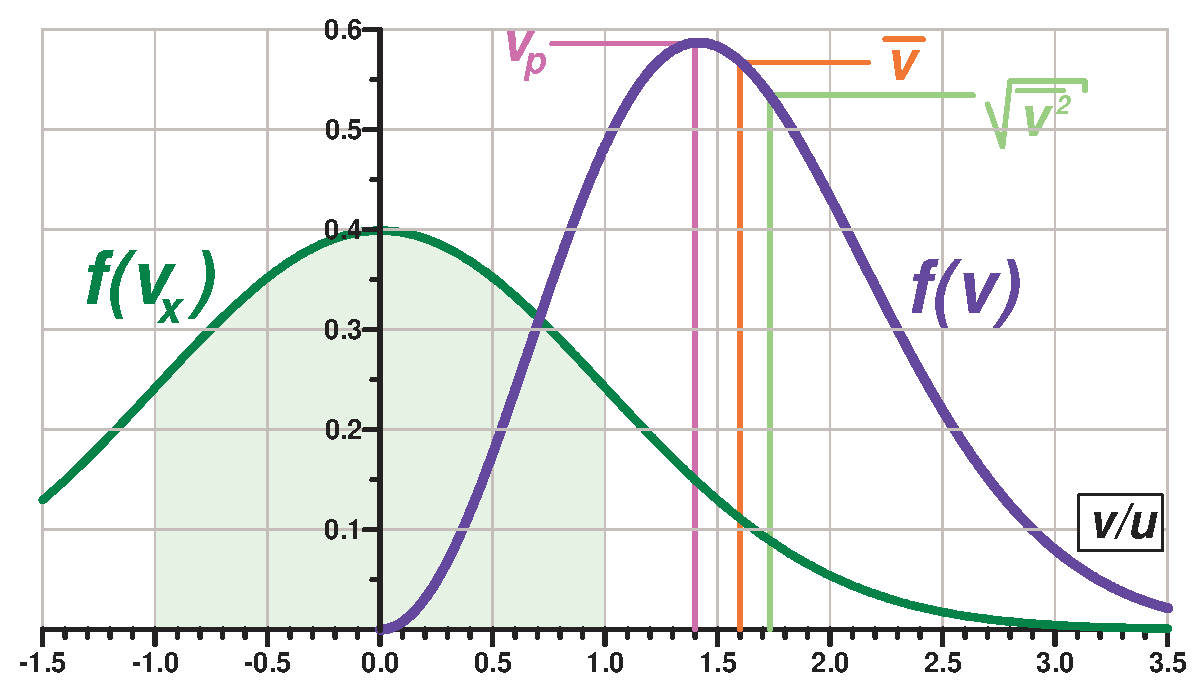
\includegraphics{GP009F04.eps}}
\end{picture}\\
Если мы вспомним, что $mv^2/2$ -- это кинетическая энергия $w$ поступа\-тель\-но\-го движения молекулы (вращение -- не в счет!!!), то $v^2=2w/m$, $dw=mv\;dv$, и можно от распределения по скоростям перейти к рас\-пре\-де\-ле\-нию по энергиям:
\begin{displaymath}
df(w)=4\pi\left(\frac{m}{2\pi kT}\right)^{3/2} \exp\left(-\frac{w}{kT}\right)\sqrt{\frac{2w}{m}}\cdot\frac{dw}{m}=
\end{displaymath}
\begin{displaymath}
=\frac{2}{\sqrt{\pi}(kT)^{3/2}}\exp\left(-\frac{w}{kT}\right)\sqrt{w}\cdot dw
\end{displaymath}
Или, выразив энергию в единицах $kT$ (то есть, введя новую переменную $\varepsilon\equiv w/kT$):
\begin{displaymath}
df(\varepsilon)=\frac2{\sqrt{\pi}}\;e^{-\varepsilon}\cdot\sqrt{\varepsilon}\;d\varepsilon
\end{displaymath}
\begin{picture}(190,100)(0,0)
 %\put(0,0){\framebox(190,100)[b]{}}
 \put(5,0){\includegraphics{GP009F05.eps}}
\end{picture}\\
Если мы нигде не ошиблись, то среднее значение $\overline{w}$ должно получаться равным $3/2kT$, что соответствует $\overline{\varepsilon}=3/2$. В этом легко убедиться:
\begin{displaymath}
\overline{\varepsilon}\equiv\frac{\int\limits_0^\infty \varepsilon \cdot e^{-\varepsilon}\cdot\sqrt{\varepsilon}\; d\varepsilon}
{\int\limits_0^\infty e^{-\varepsilon}\cdot\sqrt{\varepsilon}\; d\varepsilon}=
\frac{\left.-\varepsilon^{\frac32}e^{-\varepsilon}\right|_0^\infty-\frac32  \int\limits_0^\infty e^{-\varepsilon}\cdot\sqrt{\varepsilon}\; d\varepsilon}
{\int\limits_0^\infty e^{-\varepsilon}\cdot\sqrt{\varepsilon}\; d\varepsilon}=\frac32
\end{displaymath}

Как вы помните, плотность вероятности обнаружения молекулы со скоростью $\vec{v}$ выражалась формулой (\ref{Eq.Maxwell_1_vec{v}}):
\begin{displaymath}
df(\vec{v})
 =\frac{1}{\left(u\sqrt{2\pi}\right)^3}\cdot \exp\left(-\frac{v^2}{2u^2}\right)\cdot dV_v
\end{displaymath}
Подставив в это выражение найденное нами значение $u^2=kT/m$ и заменив ($mv^2/2$) на $E_k$, преобразуем его:
\begin{equation}\label{Eq.Maxw}
df(\vec{v})
 =\left(\frac{m}{2\pi kT}\right)^\frac32 \cdot \exp\left(-\frac{E_k}{kT}\right)\;dv_x\;dv_y\;dv_z
\end{equation}
Людвиг Эдуард Больцман обобщил этот закон распределения Максвелла на случай, когда молекулы движутся в каком-либо силовом поле (например, в гравитационном или электрическом). Тогда, согласно Больцману, надо в показателе экспоненты {\bf кинетическую} энергию $E_k$ заменить на энергию {\bf полную} = сумме кинетической и потенциальной: $E_k\rightarrow$ ($E=E_p+E_k$).

Кроме того, поскольку потенциальная энергия зависит от координат $x,y,z$, то в качестве фазового объема $dV$ надо брать не 3-, а 6-мерный ``кубик'' $dv_x\;dv_y\;dv_z\;dx\;dy\;dz$:
\begin{equation}
df= \left(\frac{m}{2\pi kT}\right)^\frac32 \cdot \exp\left(-\frac{E}{kT}\right)\;dv_x\;dv_y\;dv_z\;dx\;dy\;dz
\end{equation}
Это распределение Максвелла-Больцмана применительно к однородному полю тяжести (т.е., на не очень больших высотах) выглядит так:
\begin{displaymath}
df= \left(\frac{m}{2\pi kT}\right)^\frac32 \cdot \exp\left(-\frac{mgh}{kT}\right)\cdot \exp\left(-\frac{E_k}{kT}\right)\;dv_x\;dv_y\;dv_z\;dx\;dy\;dz
\end{displaymath}
Рассмотрим $n$ молекул, заполняющих бесконечно высокий столб газа.
Переходя от плотности вероятности к числу молекул в единице объема на какой-то определенной высоте $h$, получим:
\begin{equation}\label{Eq.Maxw-Boltz}
dn= \left(\frac{m}{2\pi kT}\right)^\frac32\cdot {\color{red} n \cdot \exp\left(-\frac{mgh}{kT}\right)}\cdot \exp\left(-\frac{E_k}{kT}\right)\;dv_x\;dv_y\;dv_z
\end{equation}
Сравнивая (\ref{Eq.Maxw}) и (\ref{Eq.Maxw-Boltz}) и желая, чтобы распределение (\ref{Eq.Maxw}) выполнялось для $n_h$ молекул, образующих слой на высоте $h$, то есть, чтобы
\begin{displaymath}
dn_h= \left(\frac{m}{2\pi kT}\right)^\frac32\cdot {\color{red} n_h} \cdot \exp\left(-\frac{E_k}{kT}\right)\;dv_x\;dv_y\;dv_z
\end{displaymath}
получаем {\bf \color{red} барометрическую формулу}:
\begin{equation}
n_h=n_0\cdot\exp\left(-\frac{mgh}{kT}\right)
\end{equation}

Ее же можно получить иначе. Знаем, что давление атмосферы -- из-за веса столба воздуха. На $\infty$ высоте давление = 0, а на какой-то высоте $h$ -- оно равно $p$. Тогда при увеличении высоты на $dh$ давление должно уменьшиться на вес этого ``кусочка'' воздуха:
\begin{displaymath}
dp=-\rho\;g\;dh
\end{displaymath}
Но плотность газа $\rho=m/V=p\mu/RT=pm/kT$. Получается диф\-фе\-рен\-ци\-аль\-ное уравнение:\vspace{-3mm}
\begin{displaymath}
dp=-p\cdot\frac{mg}{kT}\cdot dh
\end{displaymath}
Его решение -- это экспонента\vspace{-3mm}
\begin{equation}
p_h=p_0\cdot\exp\left(-\frac{mgh}{kT}\right)=p_0\cdot\exp\left(-\frac{\mu gh}{RT}\right)
\end{equation}
(поскольку $m/k=\mu/R$).\\
\begin{picture}(190,105)(0,0)
 %\put(0,0){\framebox(190,100)[b]{}}
 \put(10,0){\includegraphics{GP009F06.eps}}
\end{picture}

Прибор для определения высоты по давлению -- альтиметр.

(На самом деле, $T\neq$ const. с высотой).

\end{document}
